%% $Id: initspec.tex,v 1.7 1999/12/17 16:48:09 matt Exp $

\chapter{Initial Specification}
This specification details the initial components of the system.  The
final details of the system are left until the \emph{Technical
Specification} which appears in Chapter \ref{techspec}.

\section{System Overview}
The archive has three main functions: \emph{adding new messages},
\emph{indexing messages} and \emph{serving user requests}.  In order to
fulfil these functions the system is comprised of various components as
shown in Figure \ref{fig:overview}.

\begin{figure}[!ht]
  \begin{center}
    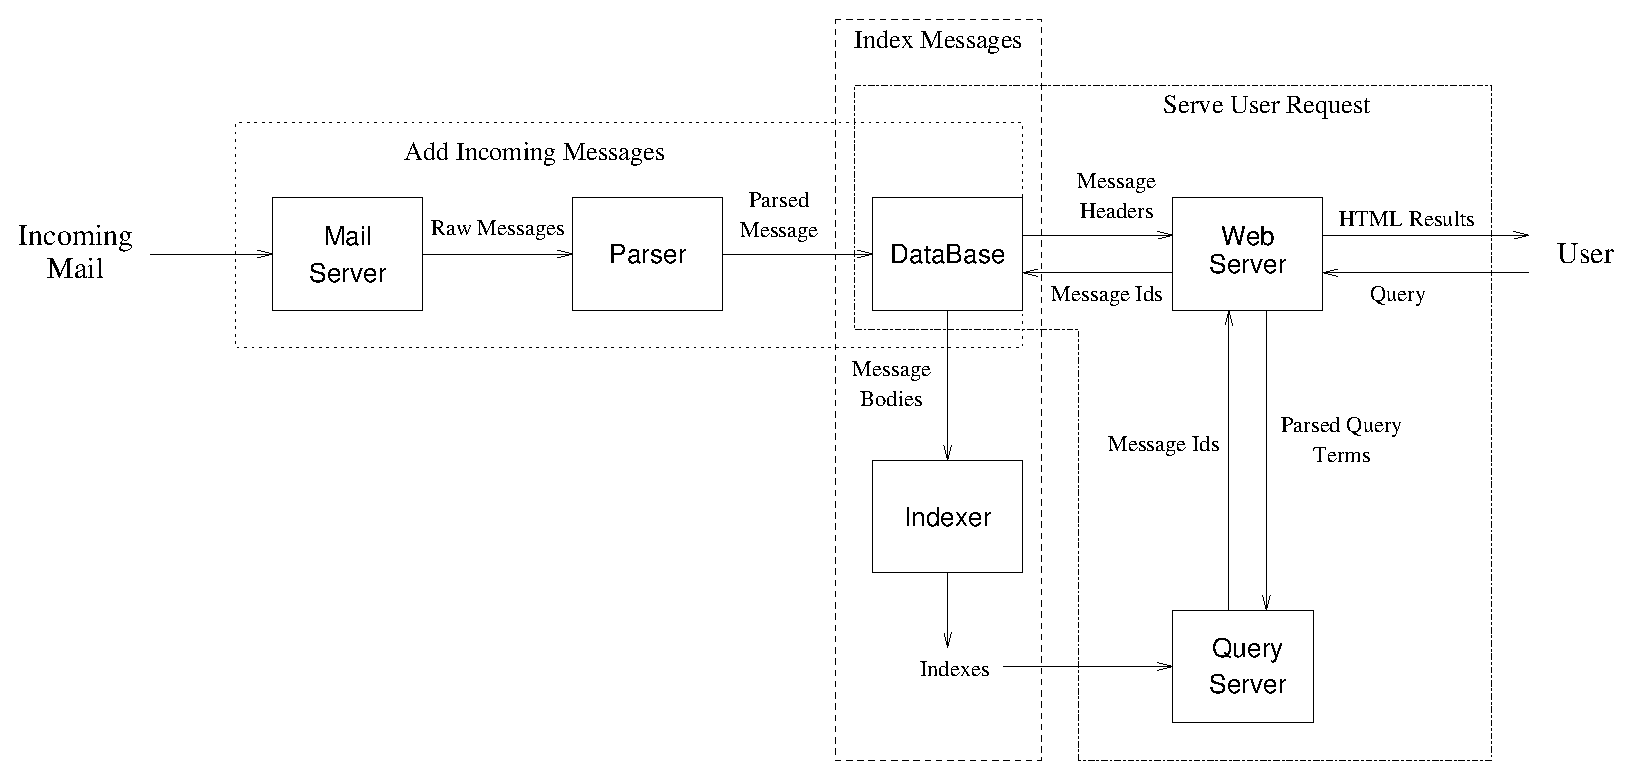
\epsfig{file=overview.eps, width=12cm}
  \end{center}
  \caption{System Overview}
  \label{fig:overview}
\end{figure}


\section{Adding new messages} 
New messages will arrive at the mail server via standard SMTP transports
from the mailing lists.  These messages will then be passed through a
parser to convert them into a suitable form to add to the database.  The
parser will also take care of adding the actual messages to the database.

\subsection{Mail Server}
The mail server will accept the messages from the mailing lists.  It must
be highly configurable, allowing messages to be piped to external
programs, and allow the creation of arbitrary addresses that are not users
according to the underlying operating system.

\subsection{Parser}
The parser must be able to take one or more messages in on standard input
from the mail server.  This means that the parser will be able to be used
like any other unix mail filter and be spawned by the mail server each
time a message appears.

During the parsing process the message will be split into its constituent
parts -- headers and body.  The relevant headers (eg. To:, From:, Date:,
Subject) will be inserted into the database along with the message body.

The message body must first be converted from any encoding that may be
used (eg. Quoted-Printable, or Base64) into plain 8bit ASCII.  If the
message is a multipart MIME message then only the parts of mime type
\texttt{text/plain} will be added.  This prevents the system from
archiving any binary attachments such as images or applications.

\subsection{Database}
The parsed messages will be stored in a database for later retrieval and
indexing.  The database must allow large \texttt{TEXT} or \texttt{BLOB}
objects to be inserted and be able to handle millions of rows efficiently.

Although, not strictly necessary it would be desirable if the database
allowed user defined functions to be coded to do particular tasks at the
server side -- eg. compression, parsing.

The database must be accessible from the parser, indexer and the web
server, hence must have an API in whatever language is going to be used
for those components.

\section{Indexing Messages}
At periodic intervals the messages must be (re)indexed.  This process
involves fetching the messages from the database and creating some sort of
index structure that can be used to quickly locate messages that match a
certain search criteria.

\subsection{Indexer}

The indexer will fetch the messages from the database and create an
inverted index of the messages.  This index will then be stored to disk
for the \emph{Query Server} to use to answer queries.

The indexer must be extremely fast and efficient on system resources.  It
is expected that the indexes will be rebuilt at least once a day, and that
there will be millions of messages in the database.  Assuming the the
average message is 2 Kilobytes, this means that the indexer must be able
to index several Gigabytes of text an hour.

As system resources are limited to the server that has been supplied, the
indexer must be able to create a full index in memory in one go, or index
chunks of the text at a time and merge the results.

The mailing lists are constantly used, thousands of messages are sent to
these mailing lists a day.  The indexer must be able to cope with
the continually growing and changing archive.

\section{Serving User Requests}
There are two main activities supported by the archive -- browsing and
searching.  This means that the archive must be able to show a
chronological list of the latest messages for a user to read through; and
be able to search through the millions of messages and return the results
of a query.

\subsection{Searching}
The search interface presented to the user must be intuitive and easy to
use.  The query entered by the user will be sent to the query server by a
script on the web server.

The query server will return a list of document ids and scores to the
script which will then fetch extra meta-data (eg. Subject, Author, List)
from the database.  The final results will be parsed by the script into
HTML and presented to the user.

\subsection{Browsing}
The user will be presented with a hierarchy of subjects and lists similar
in style to Yahoo \cite{www:yahoo}.  The catagories should be cross-linked
such that a user can can move from one related catagory to another.

Once a list has been chosen the user should be shown a view with the
most recent messages in that list.  The view should show the date the
message arrived, the author and the subject.

Clicking on a message should show the user that particular message with
the relevent headers and meta-data.  The user should be able to move
easily to previous and next messages in the list and in the subject thread
of the message.

\subsection{Customisability}
A large proportion of the target users of the archive are very technically
competent and much prefer speed and efficiency over flashy graphics and
bells-and-whistles.  On the other hand, there may be many novices who
would prefer the extra features.  The ideal situation is a system that is
customisable, so that users can make their own minds up about what they
want.

Aspects of the site that should be customisable should include:
\begin{itemize}
\item The date format (mm/dd/yy, dd/mm/yy, etc.) and the timezone.
\item The number of messages to display per screen.
\item The default lists to show when browsing.
\item Default search parameters.
\end{itemize}

The archive should keep a record of the users preferences such that when
they return to the site is is automatically displayed how they want.

\subsection{Query Server}
The query server accepts the queries from the scripts running on the web
server and returns the raw results.  The query will consist of the search
terms including any modifiers -- such as negation, the number of results
to return, and the lists to search.  The results will be a list of message
ids and their relative score according to some ranking algorithm.

The query server must return the search results within a couple of seconds
otherwise users will loose interest.

\subsection{Web Server}
The web server will be the main interface for the users to the archive.  
Therefore it must be reliable.  It must support scripting languages or
have an API to allow the connection to the Query Server.

It is possible that performing the searches on the archive may take some
time and hence the web server must be able to continue processing requests
while waiting.

\section{Misc}
\subsection{Privacy}
Not everybody wants their messages archived and there needs to be a way to
opt out of have their messages archived.  The most common method used for
archives it to set a \texttt{X-No-Archive} header in the message.  
All messages with this header will not be stored in the database.

\subsection{Platform}
The archive and indexing system must be able to run on moderate hardware.  
A server has been supplied to host the archive and indexes.  The
specifications of the server are detailed in Section \ref{serverspecs}.

% LocalWords:  ht eps unix eg multipart API ids HTML Customisability
